The event panel presents the user with a drop-down menu with a list of
available event applications. Event applications are applications
that, given the building and user supplied data inputs, will generate
a list of events (i.e., typically time-dependent loads that represent natural disasters) for the building. The following options
are available in the drop-down menu:

\begin{enumerate}
\item DEDM HRP (\Cref{subsec:dedm_hrp})
\item Stochastic Wind Event (\Cref{subsec:stochastic_wind})
\item CFD Expert (\Cref{subsec:cfd_expert})
\item Multiple Existing(\Cref{subsec:multiple_existing})
\end{enumerate}

\subsection{DEDM HRP}
\label{subsec:dedm_hrp}
This option allows users to obtain wind forces from the vortex-winds website.



\subsection{Stochastic Wind}
\label{subsec:stochastic_wind}
This option allows users to generate synthetic wind velocity time
histories for target wind loading. In order to do so, the stochastic
wind model is selected from the drop-down menu, as shown in
\Cref{fig:stochastic_wind_loading}. Depending on the model selected, the
user will be asked to enter the parameters describing the wind loading
scenario that the synthetic time history should emulate. In the
current release, users can only select the model derived by Wittig \&
Sinha (1975) \cite{wittig1975simulation}. Additionally, users can
provide a seed for the stochastic wind generation if they desire the
same suite of synthetic time histories to be generated on multiple occasions.
If the seed is not specified, a different realization of the time
history will be generated for each run based on the input
parameters. The backend application that generates the stochastic
wind loads relies on \texttt{smelt}, a modular and extensible C++
library for generating stochastic time histories. Users interested in
learning more about the implementation and design of \texttt{smelt}
are referred to its
\href{https://github.com/NHERI-SimCenter/smelt}{GitHub repository}.

All input parameters can be specified as random variables by entering
a string in the parameter field. Please note that information for the
inputs that are identified as random variables needs to be provided in
the \texttt{UQ} tab.

\begin{figure}[!htbp]
  \centering {
    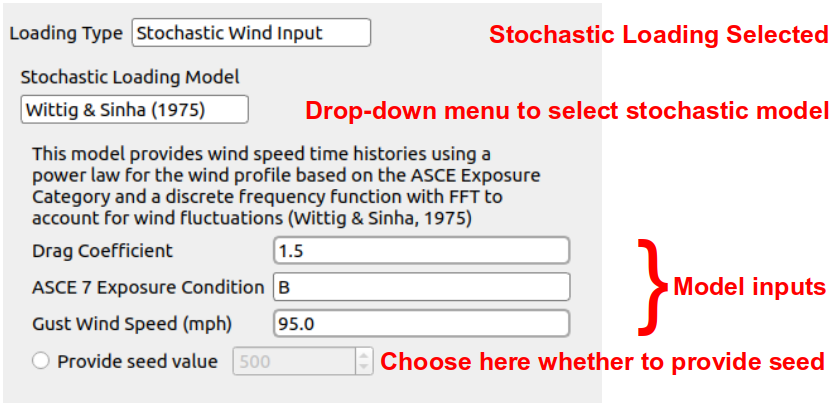
\includegraphics[width=0.8\textwidth]
    {usage/figures/stochastic_wind_loading.png} }
  \caption{Stochastic Wind Loading Event}
  \label{fig:stochastic_wind_loading}
\end{figure}


\subsection{CFD Expert}
\label{subsec:cfd_expert}
This option allows users to obtain wind forces utilizing an existing OpenFoam model 
that was uploaded to Design-Safe data depot. 
This is done by coupling the OpenFOAM model and the building model in a weak form, 
where the CFD analysis is executed first, then building forces are extracted and applied to the building model.
This initial version is limited in scope due to the following assumptions:

\begin{itemize}
    \item The OpenFOAM model has a patch with the name \textit{building} that represents the building envelope.
    \item Only horizontal forces are applied to the building model, the vertical force and moments are not considered.
    \item The building forces are extracted using the binning feature in OpenFOAM force module and thus, it is
          assumed that all the floors are of equal heights.
    \item OpenFOAM solvers supported are limited to \textit{pisoFOAM}.
    \item Meshing is performed using the \textit{blockMesh} tool.
    \item No uncertainty is considered in the CFD analysis.
\end{itemize}

It is important to note that this type of event is only supported when running the simulation at DesignSafe and 
does not run on the local computer.
The backend applications used in WE-UQ create a copy of the OpenFOAM case directory provided by the user,
then modify the post-processing stage in the case to output the forces acting on the building, for each floor level.
\Cref{fig:cfd_expert} shows input parameters required for using the CFD expert event. It is important to note
that this event requires the user to have an OpenFOAM case uploaded to DesignSafe data depot. For that reason, 
the widget is disabled when the user is not logged into DesignSafe. Once the user signs in, the widget is enabled
and the input parameters can be changed. 

\begin{figure}[!htbp]
    \centering {
        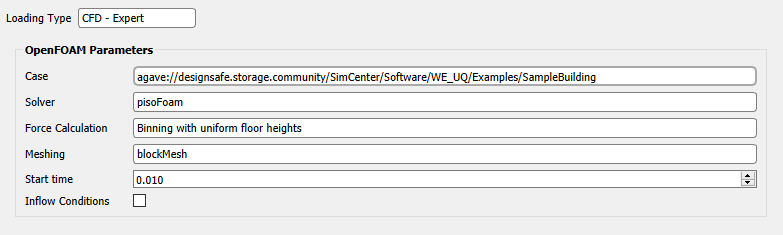
\includegraphics[width=0.8\textwidth]
        {usage/figures/cfd_expert.png} }
    \caption{CFD Expert Event}
    \label{fig:cfd_expert}
\end{figure}

There are at least 6 input parameters that needs to be provided by the user and can be summarized as follows:
\begin{itemize}
    \item \textbf{Case:} The remote path of the OpenFOAM case that was uploaded in advance to DesignSafe data depot.
    By default, this is set to an example case that is provided by the SimCebnter in the community directory.  
    \item \textbf{Solver:} The OpenFOAM solver that is used in the simulation.
    \item \textbf{Force Calculation:} The method used to calculate the forces acting on the building in the CFD analysis.
    \item \textbf{Meshing:} The meshing tool used for the provided OpenFOAM case. 
    \item \textbf{Start time:} The time in the CFD simulation to start extracting the forces on the buildings.
        Force values before that time are not used.
    \item \textbf{Inflow Conditions:} Whether or not the inflow conditions will be specified for the CFD simulation.   
\end{itemize}

If the user selects to specify the inflow conditions, the parameters for the inflow condition shown in \Cref{fig:cfd_expert_inflow}
will need to be specified.
This requires the application to download some of the case files and modify them before the simulation is started,
which is done automatically by the tool.

\begin{figure}[!htbp]
    \centering {
      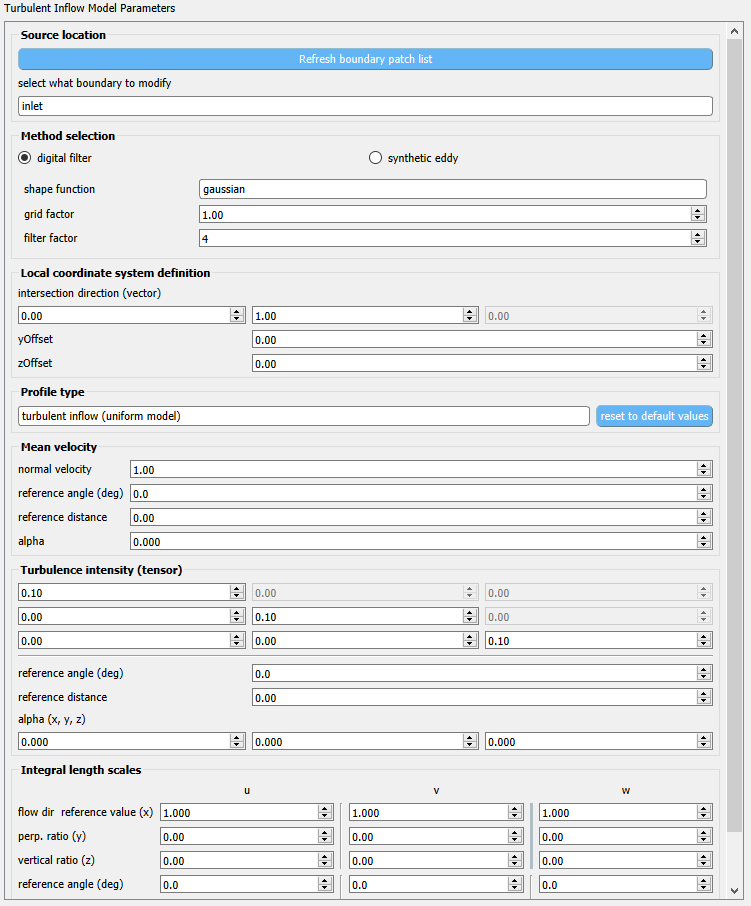
\includegraphics[width=0.8\textwidth]
      {usage/figures/cfd_expert_inflow.png} }
    \caption{Inflow Condition Parameters}
    \label{fig:cfd_expert_inflow}
\end{figure}

\subsection{CFD Template}
\label{subsec:cfd_template}
This event facilitates generating a CFD model for wind flow around a building. A template is provided to the user to generate an OpenFOAM model based on a set of parameters for mesh generation and CFD simulation. The user needs to specify the domain size, mesh size, boundary conditions, simulation parameters and the method for extracting wind forces on the building as shown in \Cref{fig:cfd_template}.

\begin{figure}[!htbp]
    \centering {
        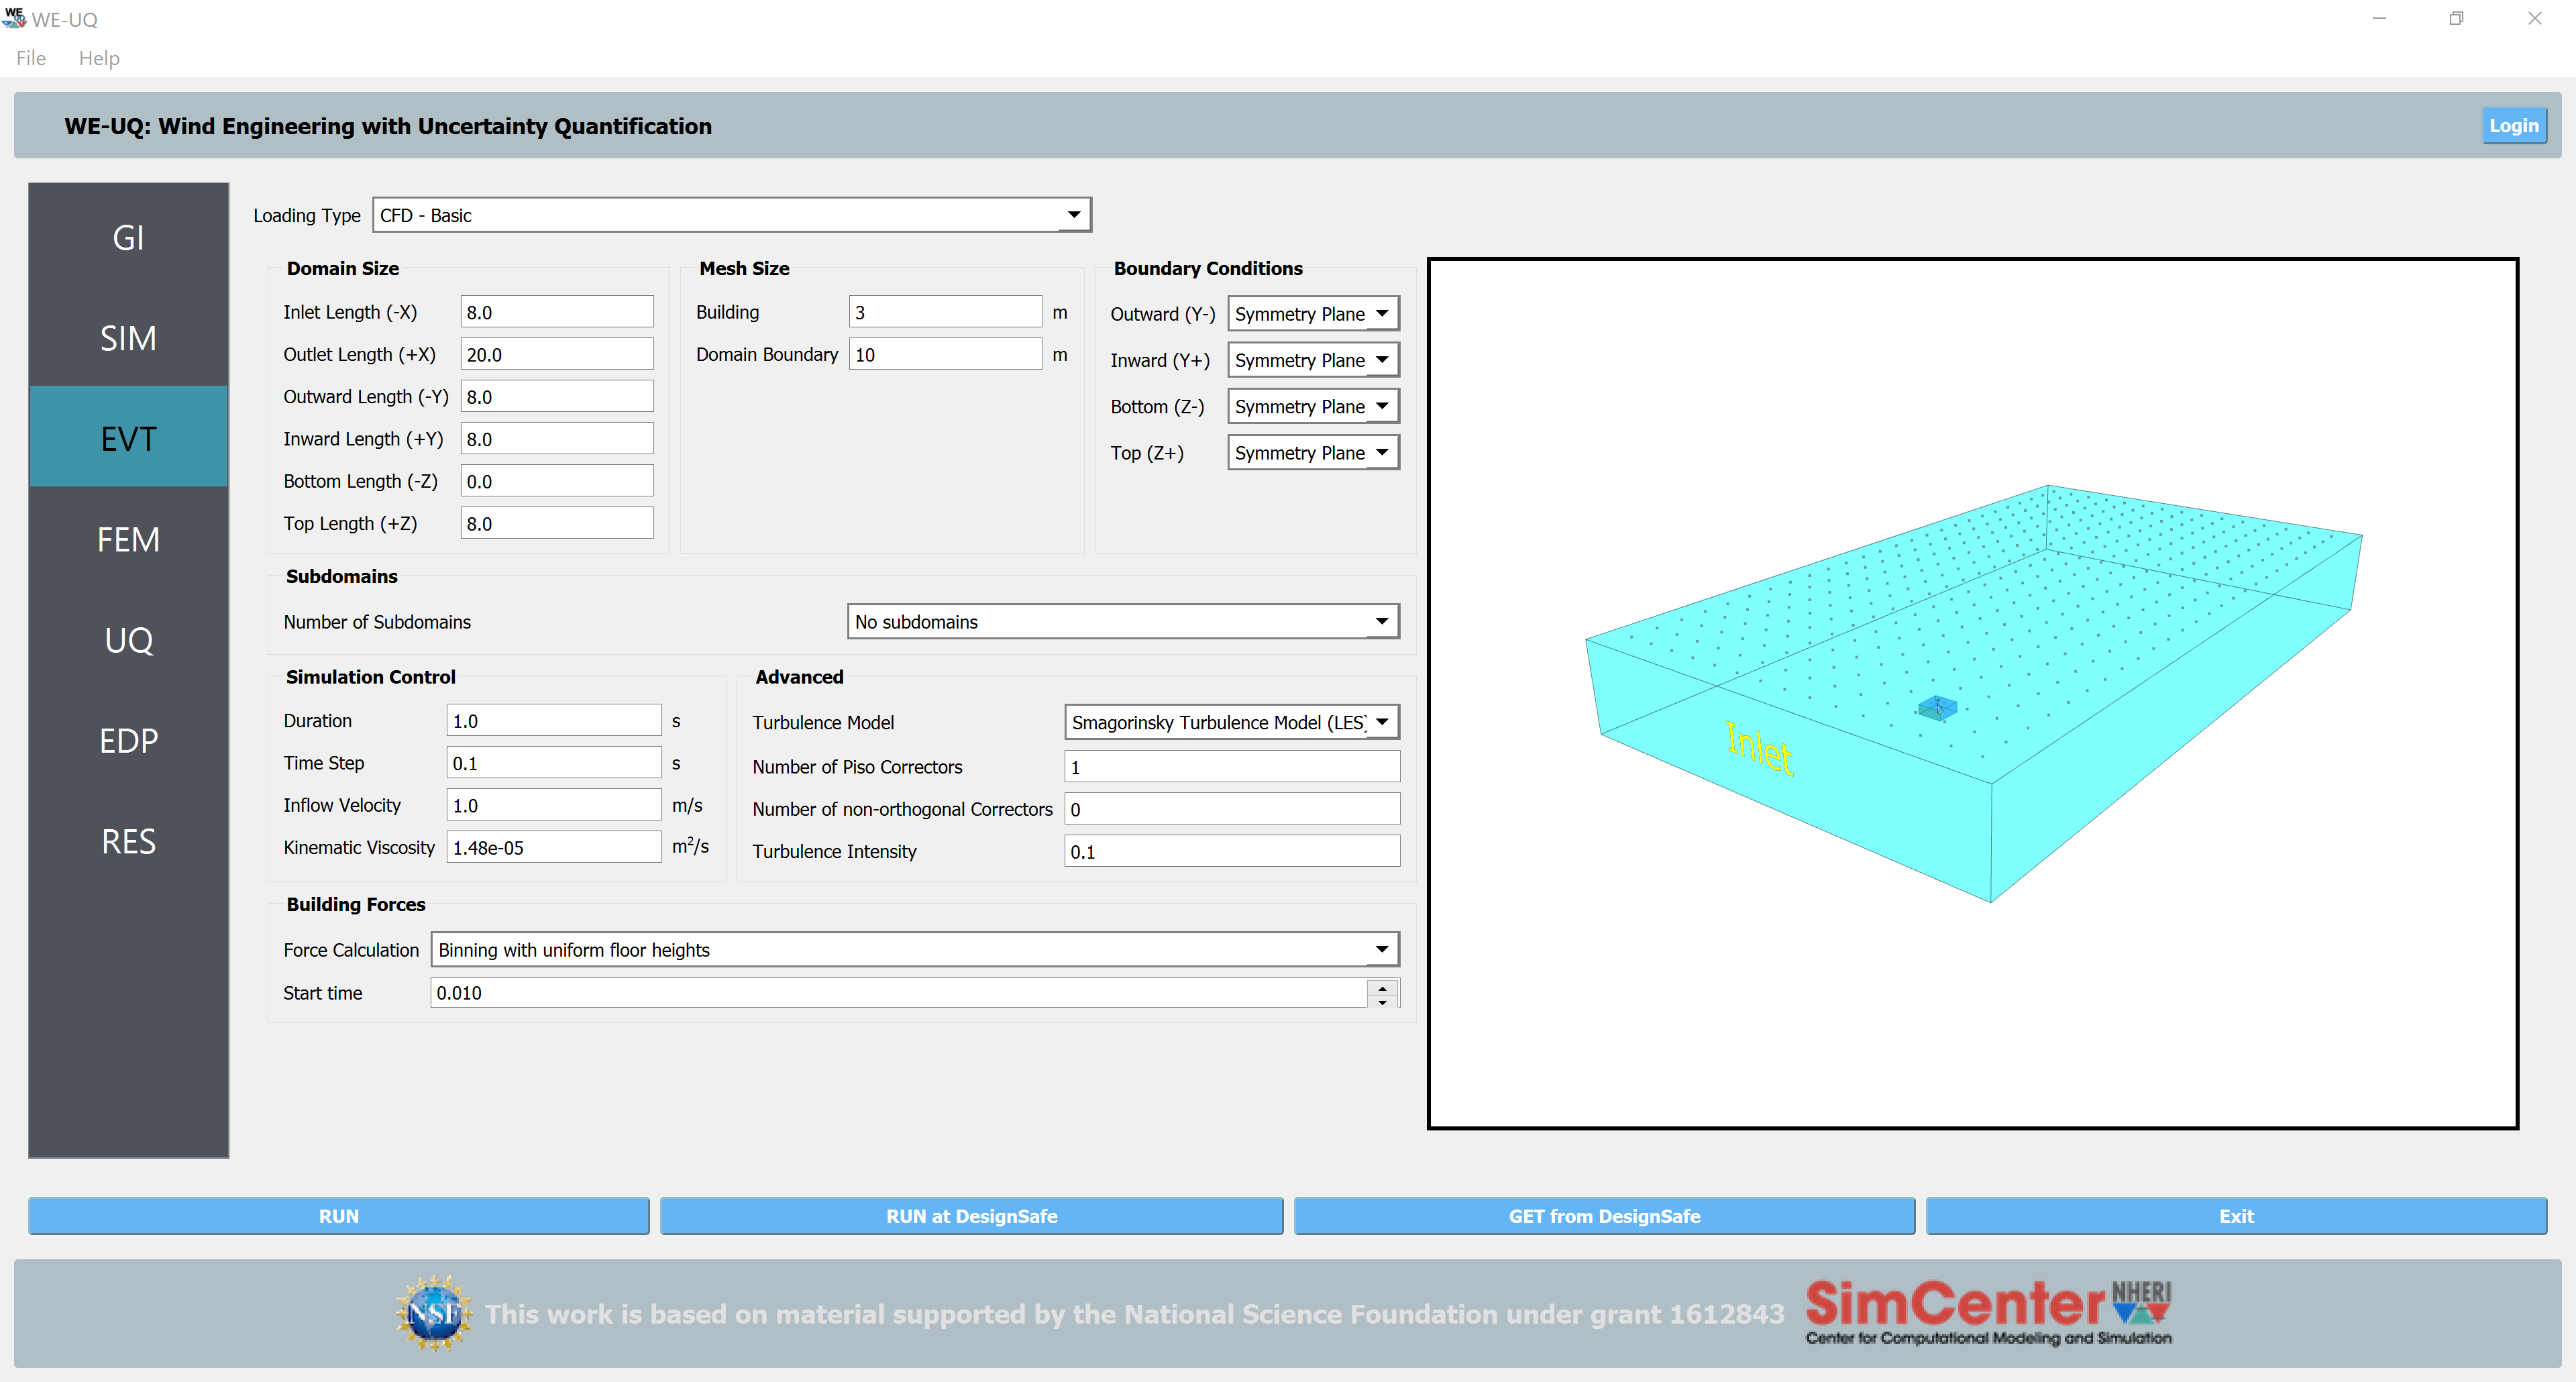
\includegraphics[width=0.95\textwidth]
        {usage/figures/cfd_template.png} }
    \caption{CFD Template Event}
    \label{fig:cfd_template}
\end{figure}

The following are the steps the user should follow to use the CFD template:

\begin{enumerate}
\item Specify the domain size in different directions using the input fields in the domain size group. It is important to note here that the size is relative to the building size. A three dimensional view is provided to allow the user to visualize the domain size. The 3D view should also indicate the location of the wind flow inlet.

\item Prescribe mesh sizes at the building surface and the outer edge of the wind field boundary. Mesh sizes are specified in meters. Users can visualize the prescribed mesh size compared to the domain and building sizes, only for the top surfaces.

\item The next step is to specify the boundary conditions on the sides, top and bottom of the domain. The user can select between wall or symmetry plane boundary conditions.

\item Optionally, the user can also specify up to three inner sub-domains. The desired mesh size and dimensions of sub-domains can be specified and they follow the same convention as the main domain.

\item Basic and advanced simulation parameters needs to be specified. The user can specify the total time, time step, wind velocity, turbulence model used in the OpenFOAM CFD simulation.

\item  Finally, the user needs to specify how the force on the building are extracted. Currently, the only method supported is to group forces on the building into bins of equal height, where each bin corresponds to a building floor. In addition, a start time for the applying the forces on the building model has to be specified, forces before that time will not be used. This allows the user to ignore force values in the beginning of the CFD simulation as they may not be accurate.

\end{enumerate}

It has to be noted that this event can only run remotely at DesignSafe-CI, and is not supported to be run on the local computer. Once the analysis is run a mesh is generated using Gmsh based on the meshing parameters specified by the user, then and OpenFOAM model is generated, analyzed and its output will be used to extract forces acting on the building, assuming the building is a rigid body. It is also important to note that intermediate meshing and CFD simulation results are available in the output archive folder for the user to inspect, if needed. 


\subsection{Existing}
\label{subsec:multiple_existing}
This panel is provided for the user to specify multiple existing SimCenter
event files.  If more than one event is specified it is done to
provide the UQ engine with a discrete set of events to choose
from\textemdash it is not done with the intention of specifying that
one event follows another.  The panel presented to the user
is shown in \Cref{fig:SC_event_panel}.

\begin{figure}[!htbp]
  \centering {
    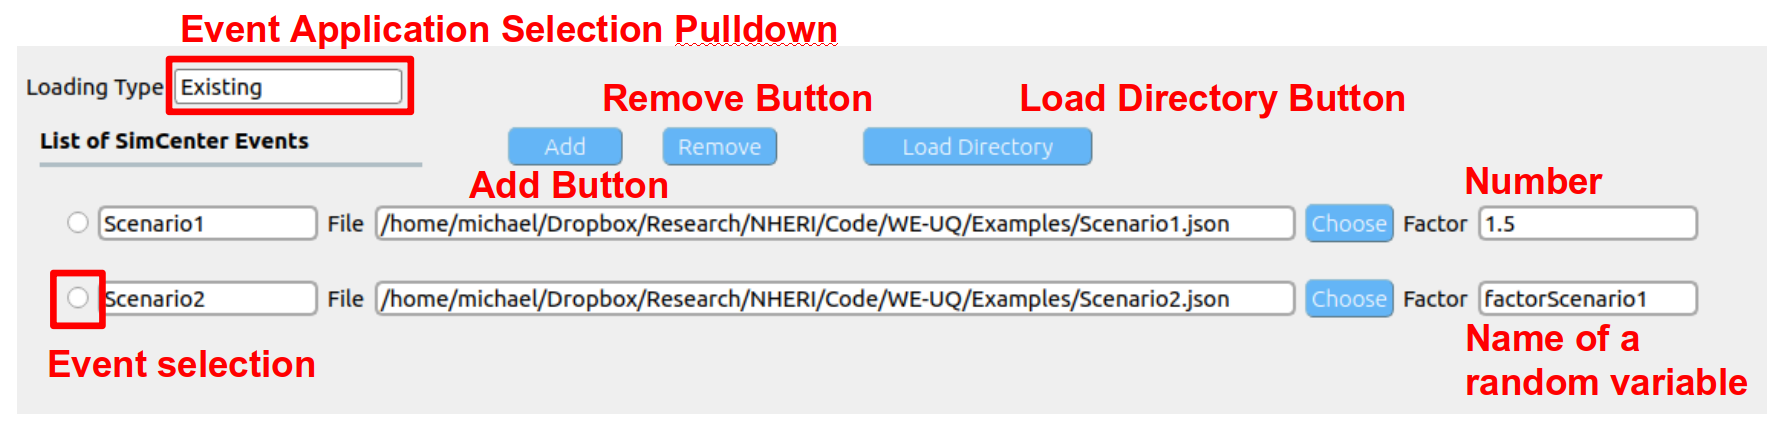
\includegraphics[width=0.8\textwidth]
    {usage/figures/weuqExisting.png} }
  \caption{Existing (SimCenter) Events }
  \label{fig:SC_event_panel}
\end{figure}

Use the \texttt{Add} button to add a new event. This adds an empty
event to the panel. Pressing the button multiple times will keep
adding events to the panel. \Cref{fig:SC_event_panel} shows the state
after the button has been pressed twice, and data entered to load
the \texttt{Scenario1} and \texttt{Scenario2} Events.

The path to the event file can be entered manually, or using
the \texttt{Choose} button for convenience. Pushing the button brings
up a typical file search screen. By default, a scale factor of 1.0 is
assigned to the event.  The user can change this to another floating
point value (DO NOT USE INTEGER), and they can define the scale factor
as a random variable by entering a variable name, such
as \texttt{factorScenario1} for the second event
in \Cref{fig:SC_event_panel}.

Note: the name of the random variable must not start with a number, or
contain any spaces or special characters, such as -, +, \%, etc.

The \texttt{Remove} button is used to remove events. To remove an
event, the user must first select events they wish to remove, which is
done by clicking in the small circle at the left side of the event
frame. All of the selected events are removed when the \texttt{Remove}
button is pressed.

The \texttt{Load Directory} button provides a convenient method to
load multiple events. All event files shall first be placed into the
same folder. We recommend to put the files in a folder of their own,
with no other files besides the wind loading events in it. After
pressing the \texttt{Load Directory} button, the user will be able to
choose the directory that contains the files, and the application will
load all event files (i.e., every file with a \texttt{.json}
extension) into the widget automatically.

Initially, every event will be given a load factor of 1.0. Load
factors can be assigned automatically by preparing
a \texttt{Records.txt} file in the directory with the events. Each
line in the \texttt{Records.txt} shall represent one event file, and
contain two comma separated values: the event file name and the
desired scale factor. The application will open that file
automatically and assign the prescribed load factors to the
events. Using a \texttt{Records.txt} file also allows users to load
only a subset of the events from a folder by listing only those in the
file. An example \texttt{Records.txt} is shown below:

\begin{verbatim}
Scenario1.json,1.5
Scenario2.json,2.0
\end{verbatim}

Random Variables: Scale factors can be defined as being random
variables by entering a string in the factor field. The variable name
entered will appear as a Random Variable in the UQ panel and the user
must specify its distribution there. If multiple events are specified,
the event itself will be also be treated as a random variable, with
each event being part of the discrete set of possible events. For this
discrete set the user does not define a distribution as this is done
automatically.

